\documentclass[11pt]{article}

\usepackage[margin=0.78in]{geometry}
\usepackage{graphicx}
\usepackage{booktabs}
\usepackage{array}
\usepackage{xcolor}
\usepackage{hyperref}
\usepackage{caption}
\usepackage{subcaption}
\usepackage{amsmath}

\hypersetup{
  colorlinks=true,
  linkcolor=blue!45!black,
  citecolor=blue!45!black,
  urlcolor=blue!45!black
}

\title{\textbf{Lumen: An Open, Differentiable, GPU-Parallel Environment for Wall-Safe Endovascular AI}}
\author{
  Colin Son, MD\\
  Seldinger, Inc.\\
  \href{https://orcid.org/0000-0002-1782-0537}{ORCID: 0000-0002-1782-0537}\\
  \href{https://github.com/SeldingerMed/seldinger-lumen}{github.com/SeldingerMed/seldinger-lumen}
}
\date{July 2026}

\begin{document}
\maketitle

\begin{abstract}
Endovascular autonomy needs simulation environments that expose the clinical signals a policy must optimize: wall contact, device state, branch selection, image observations, and safety-aware benchmark outcomes. Lumen is an Apache-2.0 endovascular AI environment built around a deformable lumen model, tube-intrinsic contact, GPU-parallel Newton/Warp execution, Gymnasium-compatible navigation tasks, synthetic fluoroscopy, luminal image generation, and replayable computer-vision datasets. The environment is designed to make wall-safe target reaching a first-class benchmark objective rather than an after-the-fact visualization. This preprint describes the system architecture, observation and dataset surfaces, reduced-order flow and device modules, and benchmark semantics used in the public release.
\end{abstract}

\section{Motivation}

Autonomous catheter and guidewire navigation has become a credible research direction for robotic endovascular intervention, with reinforcement learning, imitation learning, and inverse reinforcement learning all explored in physical and simulated vessels \cite{robertshaw2024systematic, robertshaw2024mt, jianu2022cathsim, iagn2024}. CathSim showed that an open simulator can accelerate this work by pairing robot/device simulation with reinforcement-learning tasks \cite{jianu2022cathsim,jianu2024cathsim}. Lumen extends that open benchmark surface toward the signals that are difficult to study in rigid-pipe reaching tasks: deformable-wall interaction, wall penetration, branch-route safety, paired fluoroscopic and state observations, and dataset-grade labels emitted from the same scene.

The design goal is direct: make endovascular navigation trainable as a safety-scored, reproducible AI benchmark. Lumen therefore treats the lumen as a simulated physical substrate rather than only a visual guide. Policies can be evaluated on target reach, route adherence, wall interaction, and image-observation behavior through a shared API.

\begin{figure}[t]
  \centering
  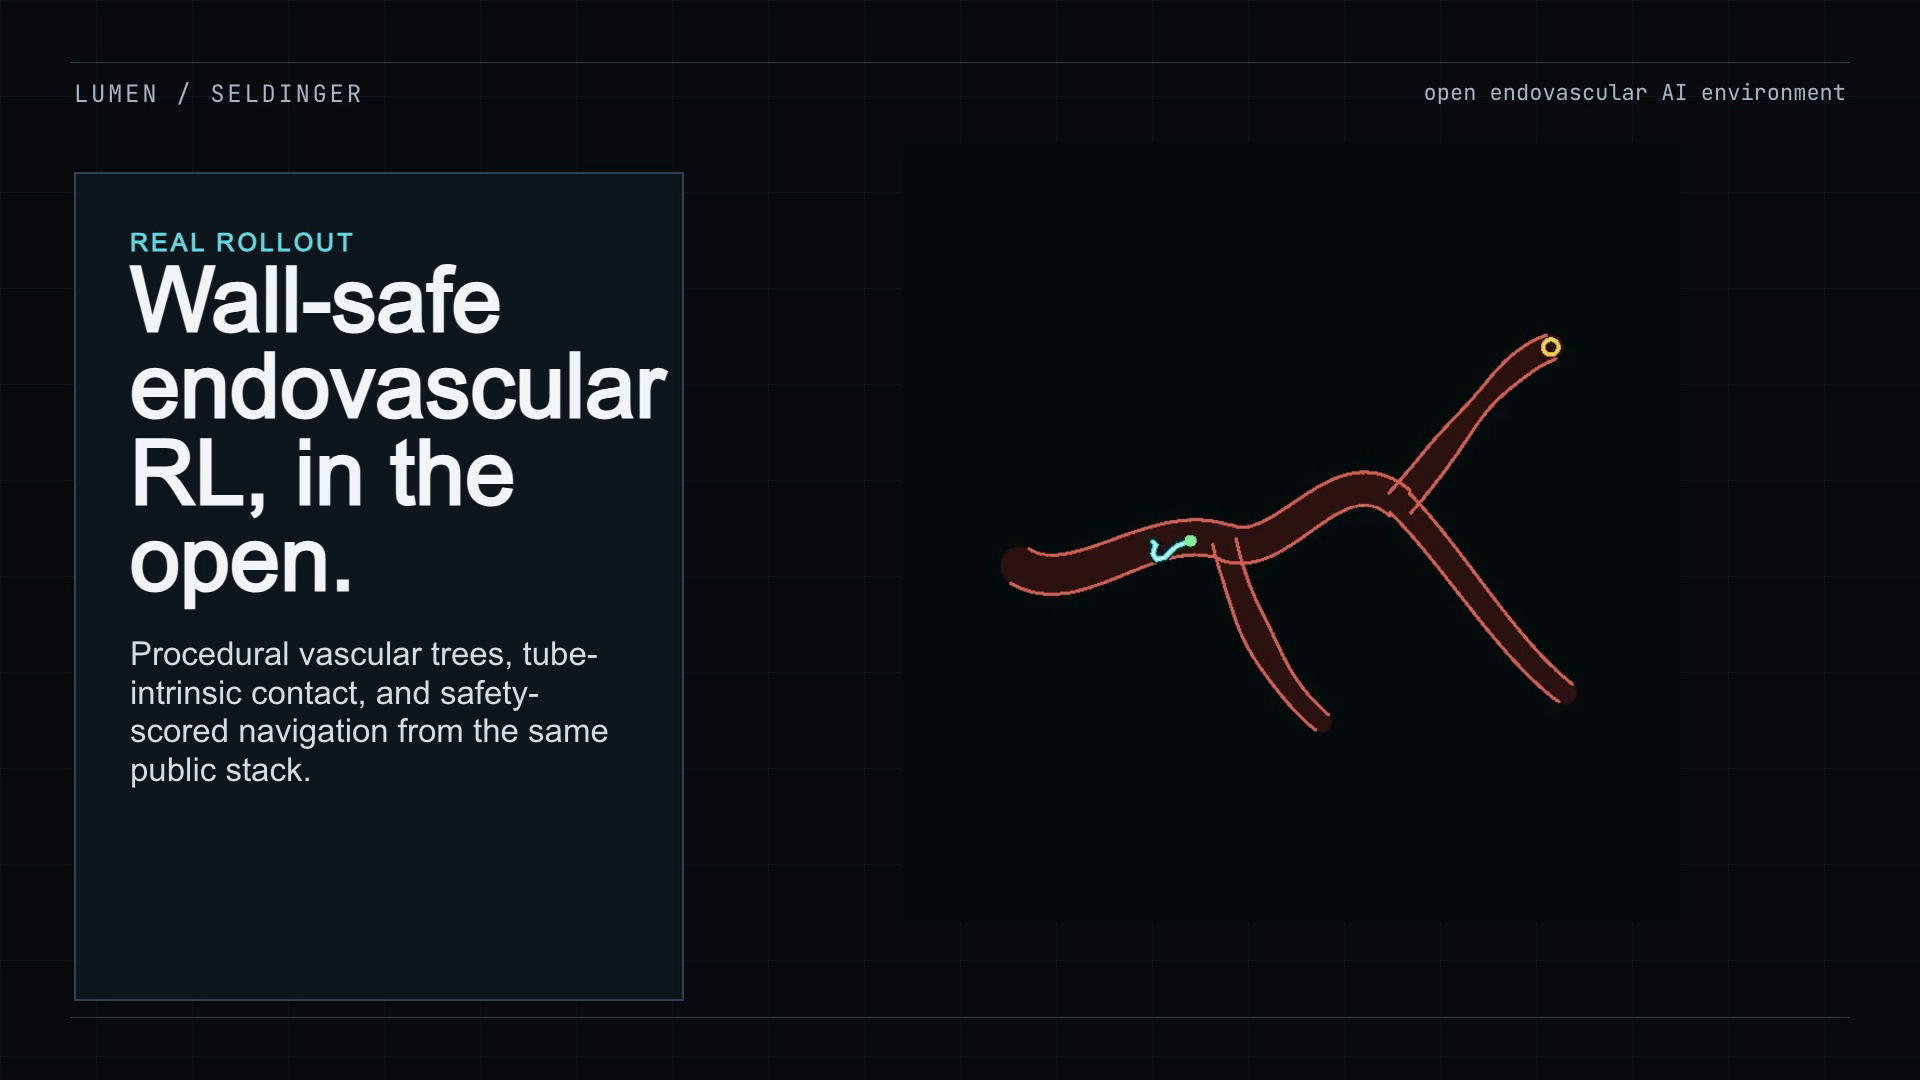
\includegraphics[width=\linewidth]{figures/figure1_overview.png}
  \caption{A real Lumen launch capture: a policy rollout in a procedurally generated vascular tree with wall-safety scoring. The launch video and public page use these real simulator-derived captures rather than generated promotional imagery.}
  \label{fig:overview}
\end{figure}

\section{System Overview}

Lumen is organized around five connected surfaces:

\begin{enumerate}
  \item \textbf{Procedural vascular cases.} Centerline trees, stenotic segments, tortuous paths, and branch targets are generated as replayable cases. This supports fast benchmark creation and deterministic reruns.
  \item \textbf{Tube-intrinsic contact and wall state.} Device progress is represented along the vessel manifold, with contact, route progress, wall penetration, torsion, and friction surfaced as environment state.
  \item \textbf{GPU-parallel simulation.} The solver path uses NVIDIA Newton/Warp-style kernels for differentiable, high-throughput simulation work \cite{warpdocs,warpgithub}.
  \item \textbf{Observation and dataset generation.} Synthetic fluoroscopy, segmentation masks, keypoints, device masks, and luminal RGB views are generated from the same scene graph.
  \item \textbf{Gymnasium-compatible RL tasks.} Navigation tasks are registered through the Gymnasium interface \cite{gymnasium2024,gym2016}, allowing existing RL tooling to treat Lumen as a standard environment.
\end{enumerate}

This arrangement follows the successful pattern of general RL benchmarks \cite{gym2016,gymnasium2024}, physics-backed control suites \cite{todorov2012mujoco}, and medical-simulation frameworks \cite{allard2007sofa,sofaweb,updegrove2017simvascular,izzo2018vmtk}, while specializing the state, observation, and scoring surfaces for endovascular device navigation.

\section{Observation Layer}

Lumen emits both state observations and image observations. The image side is deliberately multi-modal. A single scene can produce biplanar digitally reconstructed radiographs, masks for vessel and device geometry, labeled keypoints, noisy fluoroscopy, and a luminal RGB camera view. These outputs make the simulator useful not only for reinforcement learning but also for computer-vision pretraining, perception-debugging, and dataset construction.

\begin{figure}[t]
  \centering
  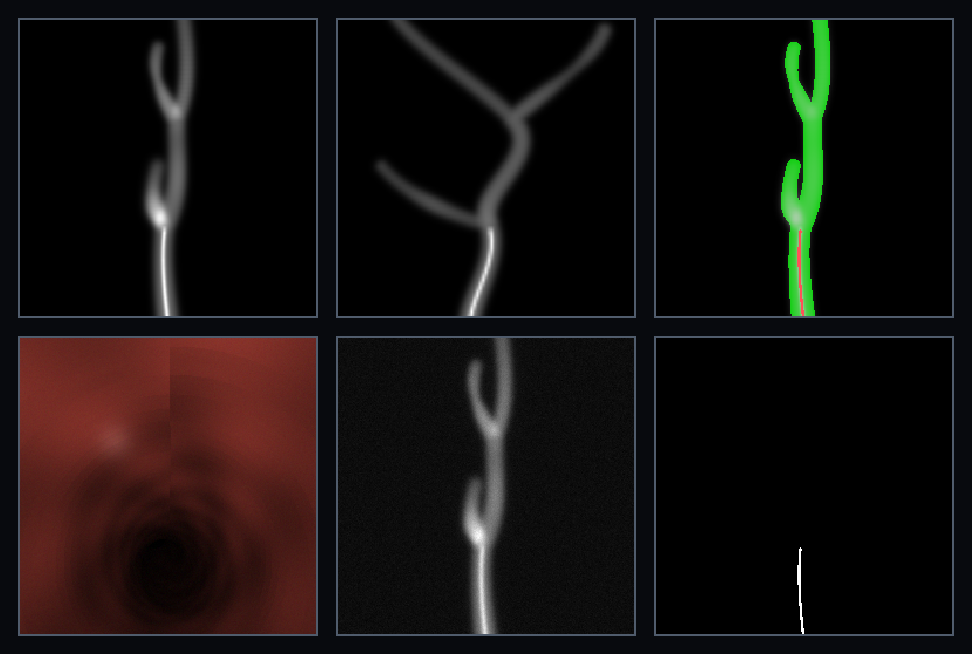
\includegraphics[width=\linewidth]{figures/figure2_multimodal.png}
  \caption{Multi-modal scene outputs from one Lumen case: biplanar fluoroscopy, vessel/device labels, luminal RGB, detector noise, and masks. The same geometry drives control state and image data.}
  \label{fig:multimodal}
\end{figure}

The dataset workflow is exposed as command-line tooling for capture, validation, indexing, and train/validation/test splitting. Episode sidecars allow users to verify that labels, masks, and replay metadata are present before a dataset is consumed by a model.

\section{Physics and Device Modules}

Lumen includes reduced-order modules for the device and vascular phenomena that should influence policy behavior. The release includes:

\begin{itemize}
  \item deformable-wall semantics inspired by arterial-wall mechanics and anisotropic constitutive modeling \cite{holzapfel2000arterial,gasser2006distributed};
  \item contact and penetration metrics reported in environment state;
  \item tortuosity, route progress, and branch-target scoring;
  \item flow-diverter effects and aneurysm inflow traces;
  \item clot-field interaction, stentriever retrieval, fragmentation, and damage bookkeeping;
  \item synthetic fluoroscopy and luminal rendering for image-observation agents.
\end{itemize}

\begin{figure}[t]
  \centering
  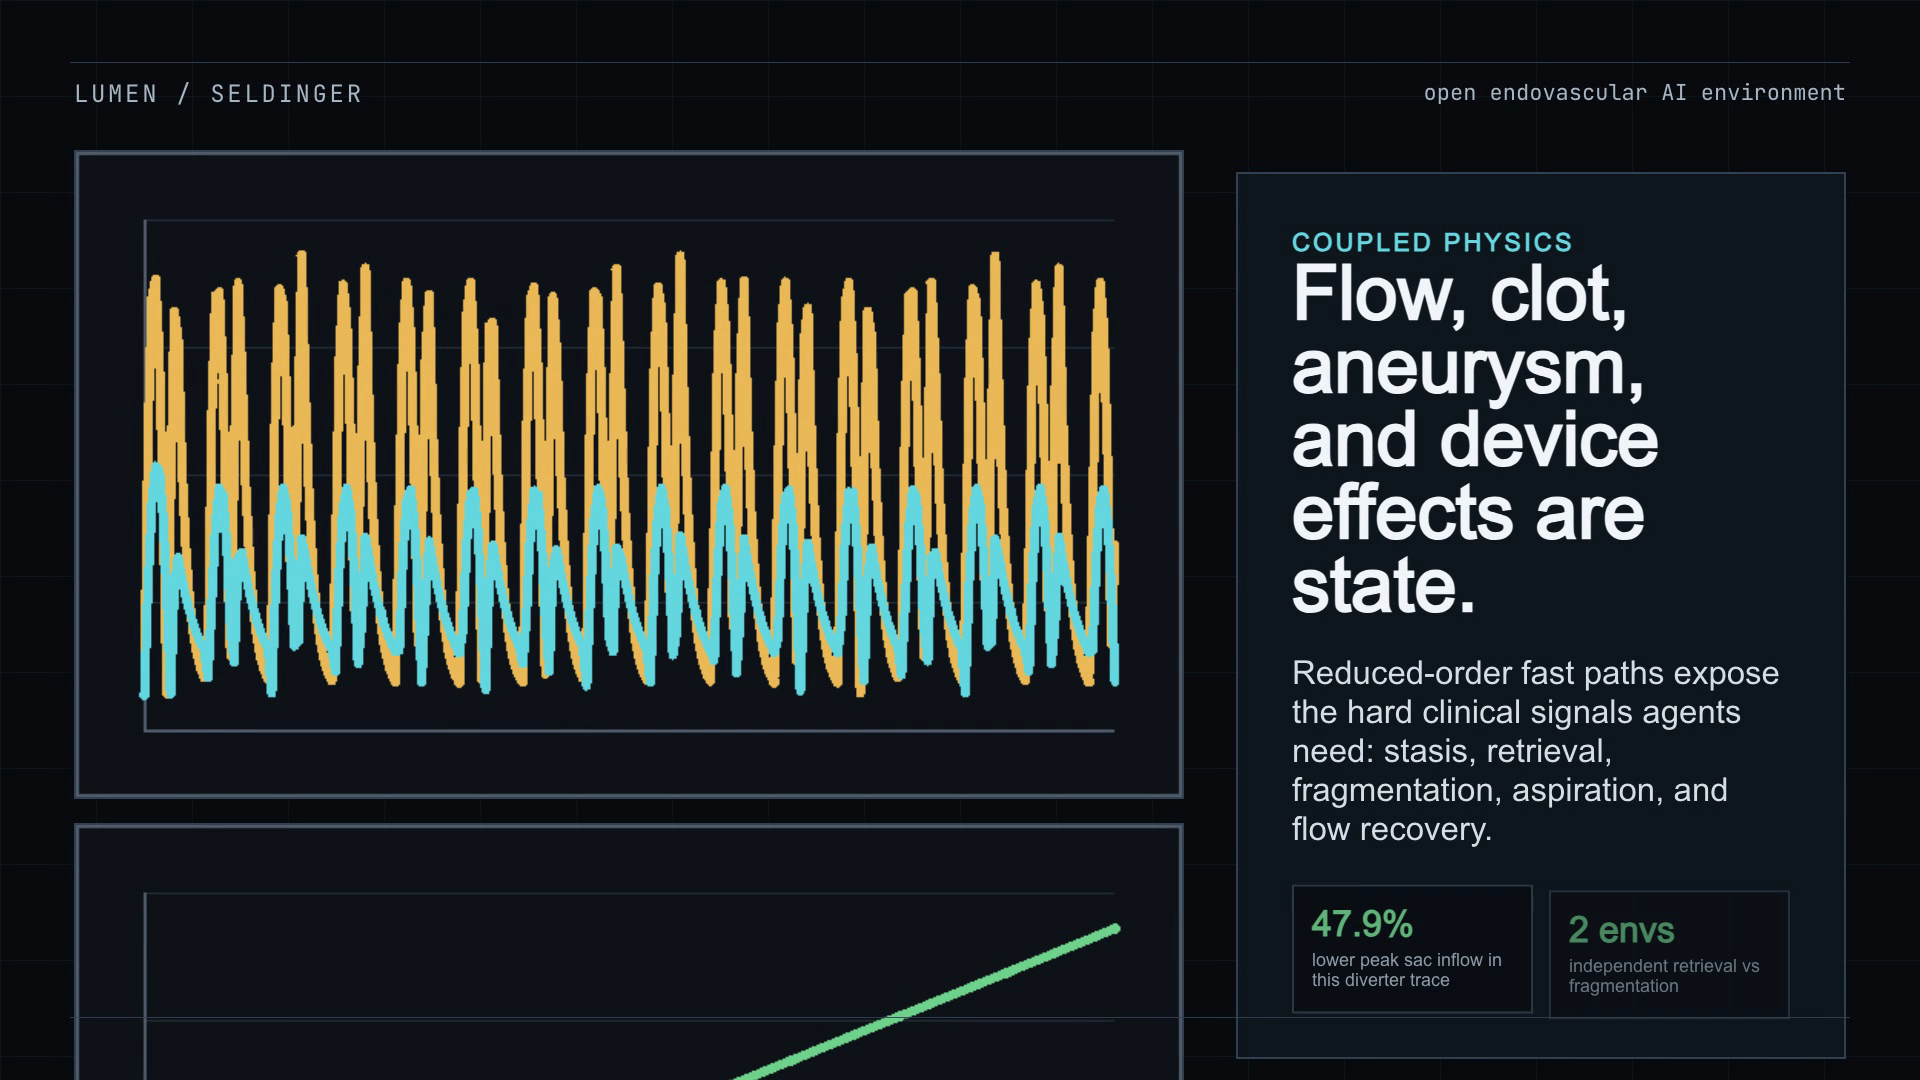
\includegraphics[width=\linewidth]{figures/figure3_physics.png}
  \caption{Advanced modules captured from the current implementation: reduced-order aneurysm inflow with a flow-diverter trace and clot/stentriever retrieval state. These modules expose clinically relevant state variables to agents and analysis scripts.}
  \label{fig:physics}
\end{figure}

The simulator is not only a renderer around a centerline. It is a benchmark substrate where contact, flow, clot/device state, and image formation can be captured together, inspected together, and reproduced from case metadata.

\section{Benchmark Semantics}

The central benchmark decision in Lumen is to rank \emph{safe success} above raw target reach. A policy that reaches a target while breaching the wall is not equivalent to a policy that reaches the target without unsafe interaction. This distinction matters for endovascular autonomy because the easiest target-reaching policy is not necessarily the most clinically meaningful policy.

\begin{figure}[t]
  \centering
  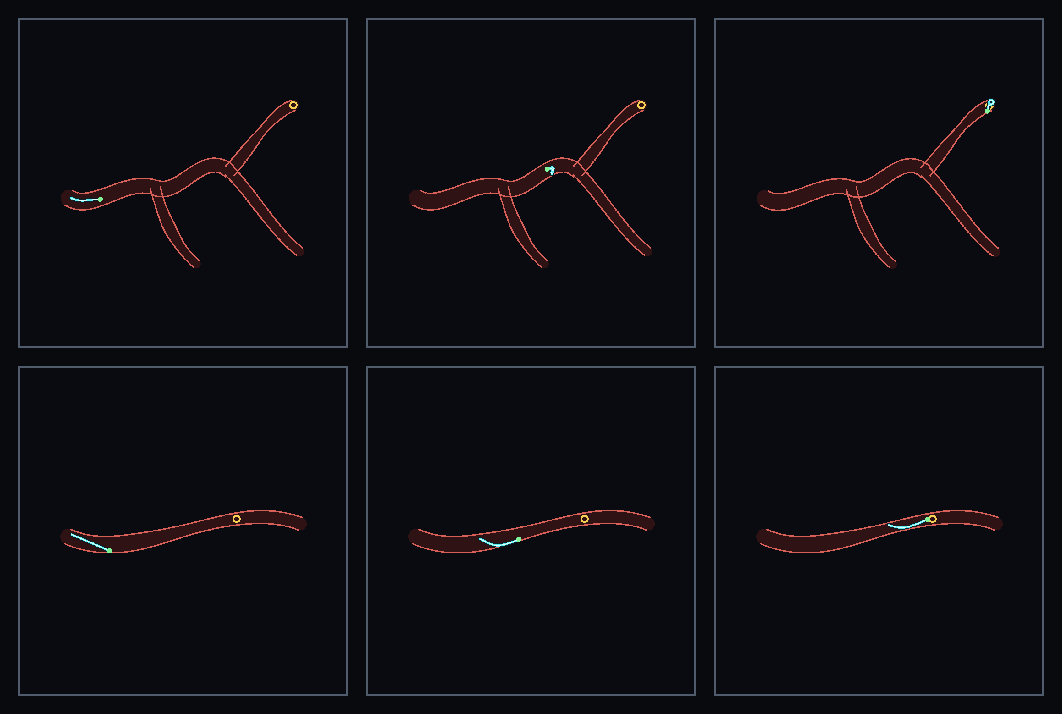
\includegraphics[width=\linewidth]{figures/figure4_benchmark.png}
  \caption{Navigation rollouts in branching and tortuous vessels. Lumen reports route progress, target reach, wall penetration, and safety status so benchmark results can distinguish safe target reach from unsafe reach.}
  \label{fig:benchmark}
\end{figure}

Lumen environments can be used with standard reinforcement-learning algorithms such as PPO and SAC \cite{schulman2017ppo,haarnoja2018sac,haarnoja2018applications}, while the environment API remains compatible with broader RL infrastructure. The benchmark output is intentionally explicit: route progress, target success, unsafe contact, wall penetration, and replay metadata are all available to downstream evaluation scripts.

\section{Positioning Relative to CathSim}

CathSim made open-source endovascular simulator research more accessible by providing an autonomous catheterization environment and validating RL tasks in simulation \cite{jianu2022cathsim,jianu2024cathsim}. Lumen is built for the next layer of benchmark pressure: deformable-wall state, wall-safety scoring, multi-modal image labels, replayable dataset tooling, and coupled endovascular state modules in one public stack.

\begin{table}[t]
  \centering
  \caption{Launch-release surface of Lumen.}
  \begin{tabular}{p{0.28\linewidth}p{0.62\linewidth}}
    \toprule
    Surface & Lumen release behavior \\
    \midrule
    RL interface & Gymnasium-registered navigation tasks and command-line benchmark runs. \\
    Safety scoring & Target reach separated from wall-safe target reach. \\
    Geometry & Procedural stenotic, tortuous, and branching vascular cases. \\
    Physics state & Tube-intrinsic contact, route progress, wall penetration, friction/torsion hooks. \\
    Image observations & Fluoro, masks, keypoints, labels, noisy detector output, luminal RGB. \\
    Dataset tooling & Capture, validate, index, split, and materialize replayable episodes. \\
    License & Apache-2.0 public repository. \\
    \bottomrule
  \end{tabular}
\end{table}

\section{Availability}

The public repository is:

\begin{center}
\href{https://github.com/SeldingerMed/seldinger-lumen}{https://github.com/SeldingerMed/seldinger-lumen}
\end{center}

The launch page, screenshots, demo video, and this preprint are published at:

\begin{center}
\href{https://seldingermed.github.io/seldinger-lumen/}{https://seldingermed.github.io/seldinger-lumen/}
\end{center}

\section{Conclusion}

Lumen provides an open endovascular AI environment where vessel navigation, wall safety, synthetic imaging, labels, and replayable benchmark artifacts are emitted from the same stack. The practical result is a stronger public substrate for studying policies that must do more than reach a coordinate: they must navigate vascular anatomy while preserving wall safety and producing interpretable image-state behavior.

\begin{thebibliography}{99}

\bibitem{jianu2022cathsim}
T. Jianu, B. Huang, M. E. M. K. Abdelaziz, M. N. Vu, S. Fichera, C.-Y. Lee, P. Berthet-Rayne, F. Rodriguez y Baena, and A. Nguyen.
\newblock CathSim: An open-source simulator for endovascular intervention.
\newblock \emph{arXiv:2208.01455}, 2022.

\bibitem{jianu2024cathsim}
T. Jianu, B. Huang, M. E. M. K. Abdelaziz, M. N. Vu, S. Fichera, C.-Y. Lee, P. Berthet-Rayne, F. Rodriguez y Baena, and A. Nguyen.
\newblock CathSim: An open-source simulator for endovascular intervention.
\newblock \emph{IEEE Transactions on Medical Robotics and Bionics}, 2024.

\bibitem{robertshaw2024systematic}
H. Robertshaw, L. Karstensen, B. Jackson, H. Sadati, K. Rhode, S. Ourselin, A. Granados, and T. C. Booth.
\newblock Artificial intelligence in the autonomous navigation of endovascular interventions: A systematic review.
\newblock \emph{arXiv:2405.03305}, 2024.

\bibitem{robertshaw2024mt}
H. Robertshaw, L. Karstensen, B. Jackson, A. Granados, and T. C. Booth.
\newblock Autonomous navigation of catheters and guidewires in mechanical thrombectomy using inverse reinforcement learning.
\newblock \emph{arXiv:2406.12499}, 2024.

\bibitem{iagn2024}
Y. Liu et al.
\newblock Image-guided autonomous guidewire navigation in robot-assisted endovascular intervention.
\newblock \emph{arXiv:2403.05748}, 2024.

\bibitem{allard2007sofa}
J. Allard, S. Cotin, F. Faure, P.-J. Bensoussan, F. Poyer, C. Duriez, H. Delingette, and L. Grisoni.
\newblock SOFA: An open source framework for medical simulation.
\newblock \emph{Studies in Health Technology and Informatics}, 125:13--18, 2007.

\bibitem{sofaweb}
SOFA Consortium.
\newblock SOFA: Open-source framework for interactive mechanical simulation.
\newblock \url{https://www.sofa-framework.org/}.

\bibitem{updegrove2017simvascular}
A. Updegrove, N. M. Wilson, J. Merkow, H. Lan, A. L. Marsden, and S. C. Shadden.
\newblock SimVascular: An open source pipeline for cardiovascular simulation.
\newblock \emph{Annals of Biomedical Engineering}, 45:525--541, 2017.

\bibitem{izzo2018vmtk}
R. Izzo, D. Steinman, S. Manini, and L. Antiga.
\newblock The Vascular Modeling Toolkit: A Python library for the analysis of tubular structures in medical images.
\newblock \emph{Journal of Open Source Software}, 3(25):745, 2018.

\bibitem{holzapfel2000arterial}
G. A. Holzapfel, T. C. Gasser, and R. W. Ogden.
\newblock A new constitutive framework for arterial wall mechanics and a comparative study of material models.
\newblock \emph{Journal of Elasticity}, 61:1--48, 2000.

\bibitem{gasser2006distributed}
T. C. Gasser, R. W. Ogden, and G. A. Holzapfel.
\newblock Hyperelastic modelling of arterial layers with distributed collagen fibre orientations.
\newblock \emph{Journal of the Royal Society Interface}, 3(6):15--35, 2006.

\bibitem{warpdocs}
NVIDIA.
\newblock Warp: A Python framework for high-performance simulation and spatial computing.
\newblock \url{https://developer.nvidia.com/warp-python}.

\bibitem{warpgithub}
NVIDIA.
\newblock NVIDIA Warp source repository.
\newblock \url{https://github.com/NVIDIA/warp}.

\bibitem{gym2016}
G. Brockman, V. Cheung, L. Pettersson, J. Schneider, J. Schulman, J. Tang, and W. Zaremba.
\newblock OpenAI Gym.
\newblock \emph{arXiv:1606.01540}, 2016.

\bibitem{gymnasium2024}
M. Towers et al.
\newblock Gymnasium: A standard interface for reinforcement learning environments.
\newblock \emph{arXiv:2407.17032}, 2024.

\bibitem{schulman2017ppo}
J. Schulman, F. Wolski, P. Dhariwal, A. Radford, and O. Klimov.
\newblock Proximal policy optimization algorithms.
\newblock \emph{arXiv:1707.06347}, 2017.

\bibitem{haarnoja2018sac}
T. Haarnoja, A. Zhou, P. Abbeel, and S. Levine.
\newblock Soft actor-critic: Off-policy maximum entropy deep reinforcement learning with a stochastic actor.
\newblock \emph{Proceedings of the 35th International Conference on Machine Learning}, 2018.

\bibitem{haarnoja2018applications}
T. Haarnoja, A. Zhou, K. Hartikainen, G. Tucker, S. Ha, J. Tan, V. Kumar, H. Zhu, A. Gupta, P. Abbeel, and S. Levine.
\newblock Soft actor-critic algorithms and applications.
\newblock \emph{arXiv:1812.05905}, 2018.

\bibitem{sutton2018rl}
R. S. Sutton and A. G. Barto.
\newblock \emph{Reinforcement Learning: An Introduction}.
\newblock MIT Press, 2nd edition, 2018.

\bibitem{mnih2015dqn}
V. Mnih et al.
\newblock Human-level control through deep reinforcement learning.
\newblock \emph{Nature}, 518:529--533, 2015.

\bibitem{lillicrap2016ddpg}
T. P. Lillicrap et al.
\newblock Continuous control with deep reinforcement learning.
\newblock \emph{International Conference on Learning Representations}, 2016.

\bibitem{todorov2012mujoco}
E. Todorov, T. Erez, and Y. Tassa.
\newblock MuJoCo: A physics engine for model-based control.
\newblock \emph{IEEE/RSJ International Conference on Intelligent Robots and Systems}, 2012.

\bibitem{coumans2021bullet}
E. Coumans and Y. Bai.
\newblock PyBullet, a Python module for physics simulation for games, robotics and machine learning.
\newblock \url{https://pybullet.org/}, 2021.

\end{thebibliography}

\end{document}
